\input{./settings}

% ====================== 个人信息 ======================
% 学院信息
\newcommand{\school}{\small{信息学部 | Faculty of Information Science}}

% 联系方式
\newcommand{\contact}{
    \scriptsize  % 使用较小字号
    \textcolor{white}{
        % 邮箱
        \faEnvelope \quad \href{523918392@qq.com}{523918392@qq.com}
        \hspace{4em}
        % 手机号
        \faPhone \quad  18711417403
        % GitHub
        \hspace{4em}
        \faGithub \quad \href{https://github.com/IceFerryLing}{https://github.com/IceFerryLing}
    }
}

%%%%%%%%%%%%%%%%%%%%
% 简历正文
%%%%%%%%%%%%%%%%%%%%
\begin{document}

% ====================== 页眉 ======================
% 包含校徽、学院名称等信息
\begin{tikzpicture}[remember picture, overlay]
    \node[anchor=north, inner sep=0pt](header) at (current page.north){
        \includegraphics[width=\paperwidth]{images/header.png}
    };
    \node[anchor=west](school_logo) at (header.west){
        \hspace{0.2cm}
        
\includegraphics[width=.34\textwidth]{images/hitsz_logo_name.png}
    };
    \node[anchor=east](school_name) at(header.east){
        \textcolor{white}{\textbf{\school}}
        \hspace{0.5cm}
    };
\end{tikzpicture}
\vspace{-3.5em}

% ====================== 页脚 ======================
% 包含联系方式
\begin{tikzpicture}[remember picture, overlay]
    \node[anchor=south, inner sep=0pt](footer) at (current page.south){
        \includegraphics[width=\paperwidth]{images/footer.png}
    };
    \node[anchor=center] at(footer.center){\contact};
\end{tikzpicture}

% ====================== 背景 ======================
% 添加校徽水印
\begin{tikzpicture}[remember picture, overlay]
    \node[opacity=0.05] at(current page.center){
        
\includegraphics[width=0.7\paperwidth, keepaspectratio]{images/hitsz_logo.png}
    };
\end{tikzpicture}

% ====================== 个人信息 ======================
\begin{figure}[h]
    \begin{minipage}{0.82\textwidth}
        \section{\makebox[\widthof{\faAddressCard}][c]{\color{HIT_Blue}{\faAddressCard}}\quad 个人信息}
        \begin{tabularx}{\linewidth}{p{\widthof{出生日期:}}Xp{\widthof{政治面貌:}}X}
            姓\ \ \ \ \ \ \ \ 名: & 周子轩 & 
            性\ \ \ \ \ \ \ \ 别: & 男  \\
            出生年月: & 2007年8月 & 
            政治面貌: & 积极分子 \\
        \end{tabularx}
    \end{minipage}
    \hspace{2em}
    \begin{minipage}{0.12\textwidth}
        \setlength{\fboxsep}{0pt}
        \doublebox{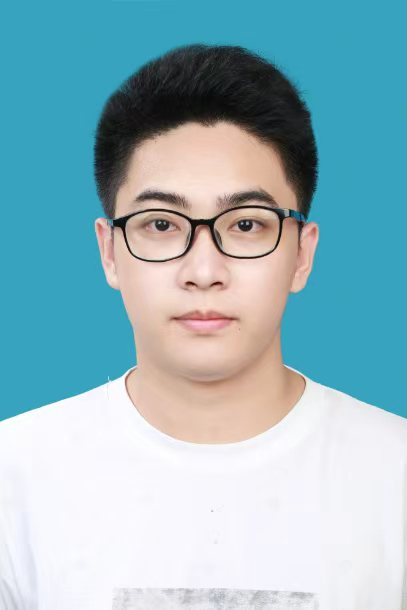
\includegraphics[width=\linewidth]{images/avatar.png}}
    \end{minipage}
\end{figure}
\vspace{-1em}

% ====================== 教育背景 ======================
\section{\makebox[\widthof{\faGraduationCap}][c]{\color{HIT_Blue}{\faGraduationCap}}\quad 教育背景}
\vspace{-0.5em}
\begin{table}[h!]
    \begin{tabularx}{\textwidth}{XXp{\widthof{2025年 -- 预计2029年6月毕业}}}
        哈尔滨工业大学（深圳） &计算机与电子通信 & 2025年 -- 预计2029年6月\\
        \textbf{学分绩: 89.89/100.00} & \textbf{学分绩排名: 155/942} \\
    \end{tabularx}
\end{table}

% ====================== 项目经历 ======================
\section{\makebox[\widthof{\faChalkboardTeacher}][c]{\color{HIT_Blue}{\faChalkboardTeacher}}\quad 项目经历}
\vspace{0.5em}
{\large{\textbf{vLLM模型推理优化比赛}}} \hfill {推理引擎 / 高性能计算}\\
参与大模型推理优化，关注吞吐、显存占用与请求调度；了解PagedAttention、continuous batching、KV Cache管理等推理引擎机制。

\vspace{0.8em}
{\large{\textbf{从零实现Transformer模型}}} \hfill {深度学习 / Python}\\
使用Python实现Embedding、Multi-Head Attention、FFN、LayerNorm等核心模块，熟悉训练循环、损失计算与推理生成流程。

\vspace{0.8em}
{\large{\textbf{金融数据处理与量化回测实验}}} \hfill {Python / 数据分析}\\
使用Pandas、NumPy完成金融数据清洗、因子计算与回测实验，围绕收益、回撤等指标评估策略表现。

% ====================== 竞赛经历 ======================
\section{\makebox[\widthof{\faTrophy}][c]{\color{HIT_Blue}{\faTrophy}}\quad 竞赛经历}
\vspace{-1em}
\begin{table}[h!]
    \begin{tabularx}{\textwidth}{Xp{\widthof{第零零负责人人人}}p{\widthof{国家级-第100名}}p{\widthof{2030年13月}}}
        \textbf{2025年全国大学生数学竞赛} & 个人 & 省一等奖 & 2025年10月 \\
    \end{tabularx}
\end{table}

% ====================== 技能特长 ======================
\section{\makebox[\widthof{\faWrench}][c]{\color{HIT_Blue}{\faWrench}}\quad 技能特长}
\vspace{0.5em}
\begin{itemize}
    \item 编程语言：熟悉\Cpp（\Cpp 11/17、内存池、线程池），熟练Python，熟悉TypeScript与Next.js
    \item 系统与高性能计算：理解CSAPP、内存管理、并发编程；掌握CUDA及Reduce、MatMul、Softmax等算子优化
    \item AI推理与深度学习：了解vLLM、PagedAttention、continuous batching；从零实现Transformer，熟悉训练与推理流程
    \item 工程与数据能力：具备AI Agent辅助开发经验，熟悉MongoDB、Git、Docker；熟练使用Pandas、NumPy进行量化回测与数据挖掘
    \item 算法基础：数据结构扎实，学习过算法竞赛知识，代码规范，学习能力强
\end{itemize}

% ====================== 所获荣誉 ======================
\section{\makebox[\widthof{\faStar}][c]{\color{HIT_Blue}{\faStar}}\quad 所获荣誉}
\vspace{-1em}
\begin{multicols}{2}
    \begin{itemize}
        \item 2025-2026学年校级优秀学生
    \end{itemize}
\end{multicols}

\end{document}
